\section{Gate-level validation}\label{sec:gates}

\subsection{Gates, corners and SPICE reference}
The five gates are standard static CMOS circuits; AND2 is a NAND2 followed by an INV and OR2 a NOR2 followed by an INV, and both are simulated in
SPICE as complete gates. Transistor widths (in multiples of $\Lmin$) are INV $W_n=1$, $W_p=2$; NAND2 $W_n=W_p=2$; NOR2 $W_n=1$, $W_p=4$
(\cref{app:assumptions}). One table of gate topologies (\texttt{src/dvdml/gates.py}) generates both the SPICE netlists and the ML prediction,
so the two always describe the same circuit.

A \emph{corner} is one random draw of $\Vdd$, temperature and the five process parameters, from the distributions of \cref{tab:sampling}; all NMOS of
a gate share one process draw and all PMOS another. The same 200 corners (\texttt{data/gates/corners.csv}) are used for every gate and input
combination and again for the test circuit, giving $18\times200=3{,}600$ SPICE runs. Inputs are ideal sources at exactly $0$ or $\Vdd$; a 0\,V source
in the ground rail makes the return current measurable. Each run records the leakage, the output voltage and the internal node voltages ($x$ between the
series NMOS of NAND2, $y$ between the series PMOS of NOR2, and the NAND2/NOR2 output $n$ inside AND2/OR2). Example netlists are in \texttt{data/netlists/gates/}.

\paragraph{Leakage definition.} The leakage of a gate is the total static current delivered by all sources at $\Vdd$ (supply plus inputs held high).
By Kirchhoff's law it equals the current absorbed by the sources at $0$\,V; both are recorded and agree.

\paragraph{Validity of the reference.} With exactly the mandated solver options, ngspice converged to an invalid operating point in 59 of the 3{,}600
runs (for example an AND2 output stuck at $7\times10^{-5}$\,V instead of $4\times10^{-8}$\,V, which made the leakage 200 times too large) and did not
converge in 66 more. Every run was therefore solved twice: with exactly the mandated options, and with one additional options line that tightens the
tolerances ($\mathrm{abstol}=10^{-15}$, $\mathrm{reltol}=10^{-9}$, $\mathrm{vntol}=10^{-12}$). The mandated result is the reference whenever the two agree within
1\,\%; otherwise the tight solve is used (\cref{tab:ref}). The mandated \texttt{.options} line is present in every netlist.
\begin{table}[H]
\centering
{\small
\begin{adjustbox}{max width=\linewidth}
\begin{tabular}{lrl}
\toprule
reference & runs & meaning \\
\midrule
mandated & 3475 & mandated options; agrees with the tight solve within 1 \% \\
tight\_only & 66 & mandated solve did not converge; tight solve used \\
tight & 59 & mandated solve disagreed with the tight solve; tight solve used \\
\bottomrule
\end{tabular}
\end{adjustbox}
}
\caption{Origin of the 3{,}600 gate SPICE reference values.}
\label{tab:ref}
\end{table}



\subsection{From transistor currents to gate leakage}\label{sec:gates_method}
For every run the ML prediction proceeds as follows (\texttt{src/dvdml/gate\_ml.py}, \texttt{scripts/07\_gate\_ml.py}):
\begin{enumerate}
  \item The SPICE-recorded output and internal node voltages and the ideal input levels give the terminal voltages $(V_d,V_g,V_s,V_b)$ of every
        transistor; with $\Vdd$, temperature, $W$ and the process parameters of the corner they form the model inputs.
  \item Each transistor is routed by its gate voltage to the ON model of its type (NMOS: $V_g>\Vdd/2$; PMOS: $V_g<\Vdd/2$) or to the OFF model, which
        predicts its four terminal currents.
  \item The currents are composed into the gate leakage in a \textbf{Kirchhoff-consistent} way.
\end{enumerate}
\textbf{Why a plain sum does not work.} In a leaking gate the ON transistors conduct only the leakage of the blocking network, at a drain--source
voltage of about $10^{-7}$\,V. Their channel current there is $g\cdot V_{ds}$ with $g\approx10^{-4}$\,S, a few $10^{-11}$\,A, and is fixed by the rest
of the circuit, not by the device. No transistor model accurate to a fraction of a percent of its ON currents can resolve it. Summing the predicted
terminal currents at the rails is therefore off by orders of magnitude (\cref{tab:estimators}).

\textbf{Kirchhoff-consistent composition.} The channel current $J$ of each ON transistor is treated as an unknown; its source current follows from
current conservation in the device, $I_s=-J-I_g-I_b$, and its gate and body currents are taken from the model. The currents of the OFF transistors
are taken from the model. Kirchhoff's current law at every internal node of the gate gives a small linear system for the unknowns $J$, solved in the
least-squares sense. The leakage is then summed once over the terminals at $\Vdd$ (supply side) and once over those at $0$\,V (ground side); the two
agree closely and their mean is reported. Only the quantities the models predict best---ON gate currents, OFF channel currents and body currents---enter
the result.
\begin{table}[H]
\centering
{\small
\begin{adjustbox}{max width=\linewidth}
\begin{tabular}{lrrrr}
\toprule
estimator & bias & median err & P95 err & mean accuracy \\
\midrule
plain sum of predicted currents, supply side & -25237.76\% & 183.55\% & 303471.20\% & -54004.89\% \\
plain sum of predicted currents, ground side & -19780.48\% & 97.14\% & 112283.84\% & -32463.97\% \\
KCL-consistent, supply side & -0.05\% & 0.20\% & 1.49\% & 99.59\% \\
KCL-consistent, ground side & 0.11\% & 0.20\% & 1.10\% & 99.66\% \\
KCL-consistent, mean of both (reported) & 0.03\% & 0.19\% & 1.20\% & 99.65\% \\
\bottomrule
\end{tabular}
\end{adjustbox}
}
\caption{Gate-level error of the ways of composing predicted transistor currents into a gate leakage (all 3{,}600 runs).}
\label{tab:estimators}
\end{table}



\subsection{Results}
\Cref{tab:gates} is the gate results table for all 18 gate and input cases; \cref{tab:bygate} summarises it per gate type and \cref{fig:gparity}
shows the parity plot of all 3{,}600 runs on log axes.
\begin{table}[H]
\centering
{\small
\begin{adjustbox}{max width=\linewidth}
\begin{tabular}{lrrrrrr}
\toprule
gate / input & SPICE median [A] & ML median [A] & bias & median err & P95 err & mean acc. \\
\midrule
INV 0 & $3.29\times10^{-11}$ & $3.25\times10^{-11}$ & -0.48\% & 0.18\% & 2.36\% & 99.44\% \\
INV 1 & $2.60\times10^{-11}$ & $2.61\times10^{-11}$ & 0.01\% & 0.37\% & 2.17\% & 99.41\% \\
NAND2 00 & $5.69\times10^{-11}$ & $5.69\times10^{-11}$ & 0.08\% & 0.09\% & 0.33\% & 99.87\% \\
NAND2 01 & $1.19\times10^{-10}$ & $1.19\times10^{-10}$ & 0.18\% & 0.18\% & 0.71\% & 99.76\% \\
NAND2 10 & $3.30\times10^{-11}$ & $3.30\times10^{-11}$ & 0.06\% & 0.11\% & 0.63\% & 99.81\% \\
NAND2 11 & $1.24\times10^{-10}$ & $1.23\times10^{-10}$ & 0.14\% & 0.31\% & 1.09\% & 99.58\% \\
NOR2 00 & $1.31\times10^{-10}$ & $1.31\times10^{-10}$ & -0.21\% & 0.12\% & 1.21\% & 99.70\% \\
NOR2 01 & $1.11\times10^{-10}$ & $1.11\times10^{-10}$ & 0.07\% & 0.19\% & 1.07\% & 99.68\% \\
NOR2 10 & $2.53\times10^{-11}$ & $2.53\times10^{-11}$ & 0.30\% & 0.42\% & 1.44\% & 99.42\% \\
NOR2 11 & $3.95\times10^{-11}$ & $3.97\times10^{-11}$ & 0.39\% & 0.38\% & 1.25\% & 99.52\% \\
AND2 00 & $9.60\times10^{-11}$ & $9.69\times10^{-11}$ & 0.03\% & 0.16\% & 1.20\% & 99.72\% \\
AND2 01 & $1.42\times10^{-10}$ & $1.42\times10^{-10}$ & 0.11\% & 0.20\% & 0.82\% & 99.73\% \\
AND2 10 & $6.90\times10^{-11}$ & $6.92\times10^{-11}$ & 0.02\% & 0.19\% & 1.19\% & 99.68\% \\
AND2 11 & $1.77\times10^{-10}$ & $1.78\times10^{-10}$ & 0.04\% & 0.21\% & 1.05\% & 99.67\% \\
OR2 00 & $1.83\times10^{-10}$ & $1.83\times10^{-10}$ & -0.14\% & 0.13\% & 1.27\% & 99.68\% \\
OR2 01 & $1.45\times10^{-10}$ & $1.45\times10^{-10}$ & -0.05\% & 0.15\% & 1.07\% & 99.70\% \\
OR2 10 & $6.81\times10^{-11}$ & $6.82\times10^{-11}$ & -0.09\% & 0.19\% & 1.38\% & 99.61\% \\
OR2 11 & $9.29\times10^{-11}$ & $9.33\times10^{-11}$ & 0.04\% & 0.23\% & 0.93\% & 99.66\% \\
\bottomrule
\end{tabular}
\end{adjustbox}
}
\caption{Gate-level results for the 18 gate/input cases, 200 PVT corners each. Error $=(I_{ML}-I_{SPICE})/I_{SPICE}$; bias is its mean, median/P95 are of its absolute value, mean accuracy $=1-$ mean absolute error.}
\label{tab:gates}
\end{table}


\begin{table}[H]
\centering
{\small
\begin{adjustbox}{max width=\linewidth}
\begin{tabular}{lrrrrrr}
\toprule
gate & runs & bias & median err & P95 err & max err & mean accuracy \\
\midrule
INV & 400 & -0.24\% & 0.28\% & 2.36\% & 5.68\% & 99.43\% \\
NAND2 & 800 & 0.12\% & 0.15\% & 0.80\% & 2.81\% & 99.75\% \\
NOR2 & 800 & 0.14\% & 0.25\% & 1.27\% & 4.94\% & 99.58\% \\
AND2 & 800 & 0.05\% & 0.19\% & 1.01\% & 2.60\% & 99.70\% \\
OR2 & 800 & -0.06\% & 0.18\% & 1.20\% & 4.60\% & 99.66\% \\
all & 3600 & 0.03\% & 0.19\% & 1.20\% & 5.68\% & 99.65\% \\
\bottomrule
\end{tabular}
\end{adjustbox}
}
\caption{Gate-level accuracy per gate type and over all 3{,}600 runs.}
\label{tab:bygate}
\end{table}



\begin{figure}[!htbp]\centering
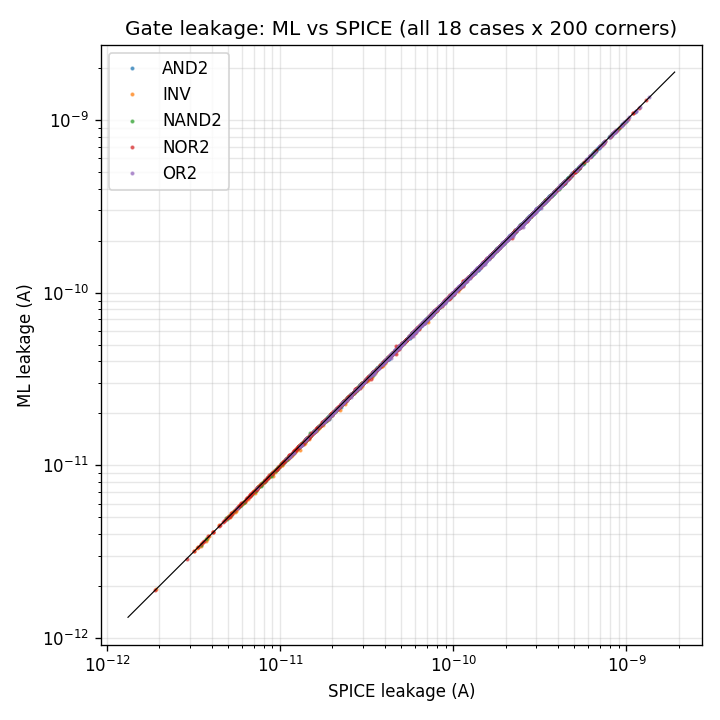
\includegraphics[width=.66\textwidth]{gate_parity.png}
\caption{ML versus SPICE leakage for all 3{,}600 gate simulations (18 cases $\times$ 200 corners), log axes; the line is $y=x$.}\label{fig:gparity}
\end{figure}

Over all 3{,}600 runs the \textbf{mean accuracy is 99.65\,\%}: median error 0.19\,\%, P95 1.2\,\%, largest error 5.7\,\%, bias $+0.03$\,\%.
Every one of the 18 cases reaches a mean accuracy of at least 99.4\,\%, and the leakage spans almost three decades
($2\times10^{-12}$ to $1.4\times10^{-9}$\,A) without visible deviation from the diagonal.
\begin{itemize}
  \item \textbf{Most accurate:} NAND2 (99.75\,\%), in particular NAND2\,00 and NAND2\,10 (median 0.09--0.11\,\%). Their leakage is dominated by gate
        tunnelling of ON PMOS devices with $V_d=V_s=\Vdd$, which the PMOS ON model predicts to within 0.1\,\%.
  \item \textbf{Least accurate:} INV\,0, INV\,1 and NOR2\,10 (mean accuracy 99.41--99.44\,\%). These are the cases in which a single OFF transistor
        carries a large share of the leakage---the OFF NMOS of INV\,0, the OFF PMOS of INV\,1 and the upper OFF PMOS ($W=4\Lmin$) of the NOR2 stack
        in NOR2\,10---so the error of the OFF channel-current model (1--3\,\%) is weighted more strongly than in the other gates
        (\cref{sec:errors}).
  \item AND2 and OR2 are about as accurate as NAND2 and NOR2 (99.66--99.70\,\%): the two stages are composed together and their errors partly average.
\end{itemize}
The internal node voltages used by the ML side are, by construction, those recorded by SPICE (step 1 above, as the assignment prescribes), so for every
run the internal node voltages of the SPICE and the ML evaluation are identical; both are stored with the run results
(\texttt{results/gates/gate\_runs\_ml.csv}, per-device inputs and predicted currents in \texttt{gate\_devices\_ml.csv}).
